\documentclass[12pt]{article}

% Language setting
% Replace `english' with e.g. `pathspanish' to change the document language
\usepackage[english]{babel}

% Set page size and margins
% Replace `letterpaper' with`a4paper' for UK/EU standard size
\usepackage[a4paper,top=2cm,bottom=2cm,left=3cm,right=3cm,marginparwidth=1.75cm]{geometry}

% Useful packages
\usepackage{amsmath}
\usepackage{graphicx}
\usepackage[colorlinks=true, allcolors=black]{hyperref}


%title
\title{\underline{AutoPylot}}
\date{}

\author{%
    \\
    Maxime Ellerbach \\
    Mickael Bobovitch \\
    Alexandre Girold \\
    Maxime Gay \\ \\
    Group: Autonomobile 
    }

\begin{document}
\maketitle
\newpage

\tableofcontents
\newpage

\section{Introduction}

\subsection{Project nature}
Autonomous cars will likely dominate our roads in a relatively close future,
with this project, we aim to have a first approach to such a complex problem.
We will be using a 1:10 scale radio controlled car modified to integrate onboard computer such as a raspberry pi and some sensors.

\subsection{State of the art}

In this section, we will try to see what was previously made in this sector of industry.
It would not be realistic to compare our 1:10 project to real sized cars such as Tesla's, simply because in a racing environnement,
we don't need to deal with such an amount of safety: pedestrian detection, emergency braking, speed limit detection and other.
So we will only see miniature autonomous racing framework that we would likely race against.\\

The most known is called "DonkeyCar", created by Will Roscoe and Adam Conway in early of 2017. Most of the models trained with DonkeyCar are behavior cloning models, meaning models that tries to replicate the behavior of a driver. This methods uses a big amount of images (input) associated to steering angles and throttle (output), it requires the user to drive the car (collect data) prior to training the model: no examples means no training. The lack of training data often leads to the car leaving the track.\\

One other framework worth looking at is one created by Nvidia called "JetRacer" released in 2019. It uses a different approach from DonkeyCar where the user annotates the images by hand by clicking on where the car should go. The model used is similar to what DonkeyCar uses meaning a Convolutional Neural Network with one input (the image) and two outputs, one for the steering angle and one for the throttle to apply.

\section{Objectives}

\subsection{Final objectives}
Our main objective is to make our car race against other cars and win the race !
This will require multiple intermediate milestones:
\begin{itemize}
\item Being able to send scripted controls to the motor and servo.
\item Being able to drive the car manually using a controller.
\item Develop a way to gather images and annotations and store them in a stuctured way, for example sorted by date.
\item Process those data before feeding them to the neural network.
\item Being able to train a convolutional neural network using those data.
\item Tweak the architecture and the parameters of the chosen model to acheive the best results.
\item Test in real life the model.
\item Race against other !
\end{itemize}
Once all of that is done, we will start our optional objectives that will enable better racing and better understanding of the car's environnement.

\subsection{Optional objectives}
To be able to go faster and increase the reliability of our car's driving, we will need to add some features to our project. \\

One good feature would be to have a model that takes into account the speed of the car. As we all know on a real car, we don't steer the same way when going at 10km/h and going at 90km/h. This input extension could bring more stability to our model.
To go faster, it would also be great to be able to differenciate turns from straight lines and even braking zone before the turn. \\

One of the challenges racing implies is overtaking. Overtaking is a very complex manoeuver. First we obviously need to be faster than the car ahead, we could assure that by detecting the successive positions of the car ahead on the image. If the car is getting closer, it's Y coordinate will come closer to the bottom of our image. Also, we cannot overtake if we have no room for that, that means we have to detect a gap on the left or the right of the car before initiating the overtake. Once we decided on what part of track we will overtake, we still need to get ahead of the opponent's car. We could acheive that by forcing the model to drive on the left or right part of the track for a given amount of time.

\subsection{Motivations}

\section{Technical specifications}

\subsection{Hardware}
On the hardware side, we already have a working car containing:
\begin{itemize}
\item A RaspberryPi 4. It is used for heavy computations like image processing, model inference, and other. Most of our programs will run on this device.
\item A USB camera. Connected to the RaspberryPi, this camera will be our main source of data.
\item An Arduino Mini. It is used for the low level, it handles commands sent by the RaspberryPi on the serial port, processes them and send PWM signals to both the ESC (Electronic Speed Controller) and servo motor.
\item An Electronic Speed Controller (or ESC). It is used to drive the motor, it receives  from the arduino a PWM signal (Pulse width modulation).
\item A Servo moto. Just like the ESC, it receives a PWM signal
\item A Speed sensor. This sensor will be usefull for our optional objectives that will require a speed feedback. This sensor is read by the arduino, then the data is sent to the RaspberryPi over the serial port.
\end{itemize}

Here is a schema of the current hardware setup we will be using:

\rotatebox[origin=c]{-90}{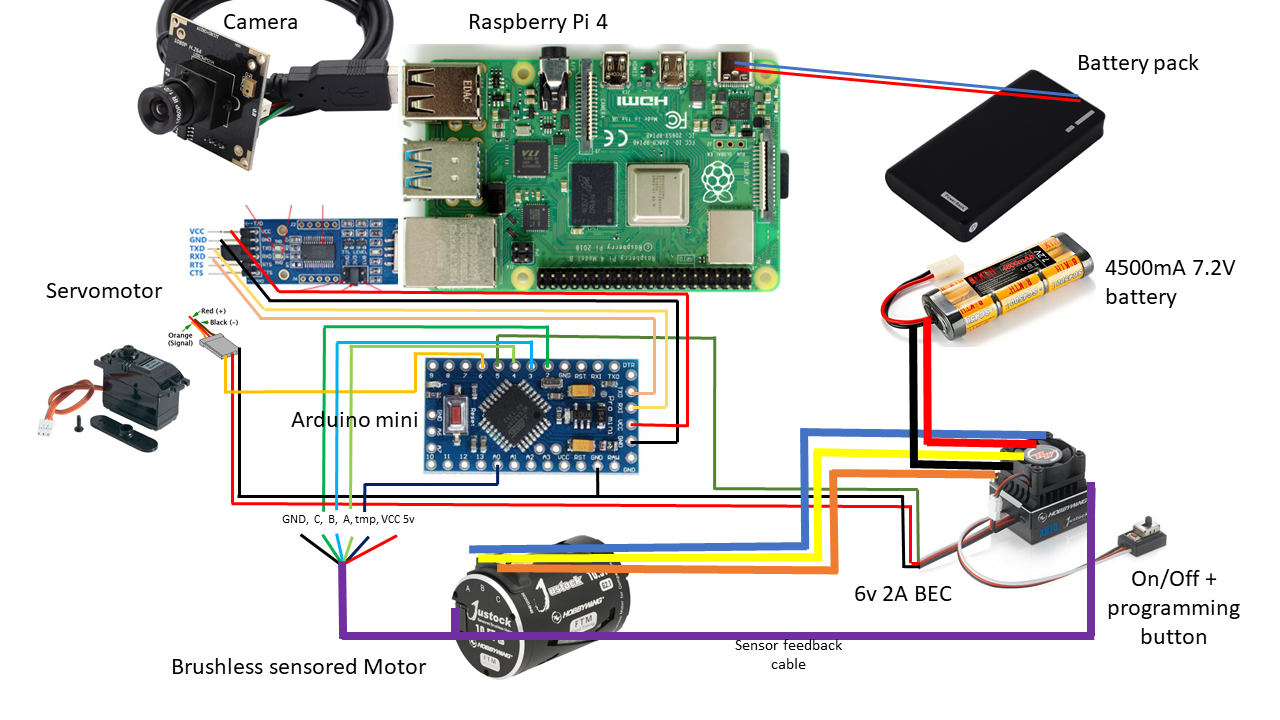
\includegraphics[width=25cm]{schema.png}}

\subsection{Software}
- data generation / gathering
- what software parts we will need

\subsection{Constraints}
- weight
- language: python
- autonomous navigation
- data ?
- framerate, efficiency of the algorithm
- safety

\section {Planning}
\rotatebox{-90}
{
\begin{tabular}{|c|c|c|c|c|c|}
  \hline
  Race 1 \tiny{(29/01)} & Race 2 \tiny{(26/02)} & Race 3 \tiny{(19/03)} &  Race 4 \tiny{(16/04)} &  Race 5 \tiny{(14/05)} &  Race 6 \tiny{(04/06)} \\
  \hline
  0 & 1 & 2 & 3 & 4 & 5 \\
  \hline
  6 & 7 & 8 & 9 & 10 & 11 \\
  \hline
\end{tabular}
}

\section {Task allocation}
\begin{tabular}{|l|c|c|c|c|}
  \hline  Tasks & Mickael B. & Maxime G. & Alexandre G. &  Maxime E.\\
  \hline  Do Something & x &  &  & x \\
  \hline  Do Something else &  & x & x & \\
  \hline
\end{tabular}

% Maybe write later
\section {Conclusion}

\end{document}